
\documentclass{beamer}

\usetheme[subsectionpage=progressbar]{metropolis}

\usepackage{tikz}
\usetikzlibrary{babel}
\usetikzlibrary{arrows,shapes,positioning,shadows,trees,calc,fit}
\usetikzlibrary{overlay-beamer-styles} % 'visible on' option for nodes
\usepackage{adjustbox}


\title{Résolution de niveaux du Sokoban}
\date{\today}
\author{PoulpoGaz, darth-mole}
\institute{Candidat n° 012345}

\usepackage{graphics}
\graphicspath{{../../assets/}}
\usepackage{subcaption}

% French language support (e.g. date format)
\usepackage[french]{babel}
\usepackage[T1]{fontenc}
\usepackage{lmodern} % for missing fonts (e.g. italic in titles)

\newenvironment{customtree}{
    \begin{tikzpicture}
        [sibling distance = 10em,
        level distance = 6em,
        every node/.style = {
            shape=rectangle,
            draw,
            scale=0.85
        },
        dot/.style = {
            font = \Large
        },
        edge from parent path = {
            (\tikzparentnode) |-                          % Start from parent
            ($(\tikzparentnode)!0.5!(\tikzchildnode)$) -| % make an ortho line to mid point
            (\tikzchildnode)                              % make another ortho to the target
        }
    ]
}{
    \end{tikzpicture}%
}

\begin{document}

    \maketitle

    \begin{frame}{Plan}
        \tableofcontents%[hideallsubsections]
    \end{frame}

    \section{Le jeu du Sokoban}
        \begin{frame}{Le jeu du Sokoban}
            \begin{columns}
                \begin{column}{0.3\textwidth}
                    \begin{figure}
                        \centering
                        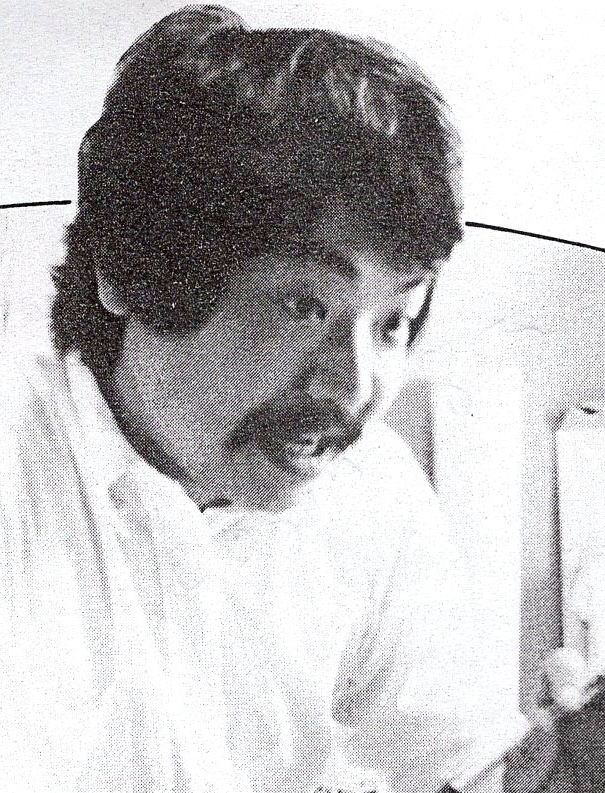
\includegraphics[width=\columnwidth]{creator.jpg}
                        \caption*{Hiroyuki Imabayashi}
                    \end{figure}
                \end{column}
                \begin{column}{0.7\textwidth}
                    \begin{figure}
                        \centering
                        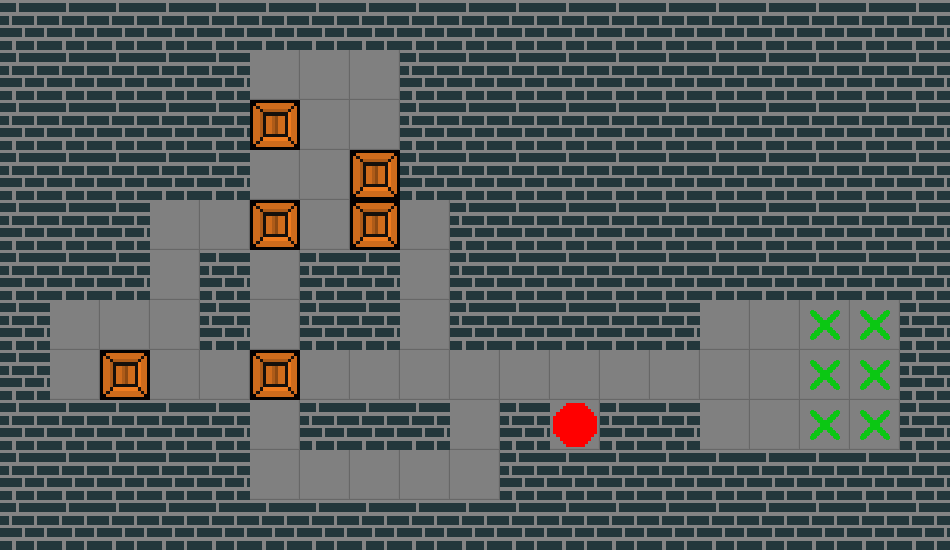
\includegraphics[width=\columnwidth]{level_example.png}
                        \caption*{\textit{Original \& extra}}
                    \end{figure}
                \end{column}
            \end{columns}
        \end{frame}

        \begin{frame}{Règles}

            \begin{columns}
                \begin{column}{0.5\textwidth}
                    \only<1-2>{
                        \begin{figure}
                            \centering
                            \begin{tikzpicture}
                            \node[anchor=south west, inner sep=0] (image) at (0,0) {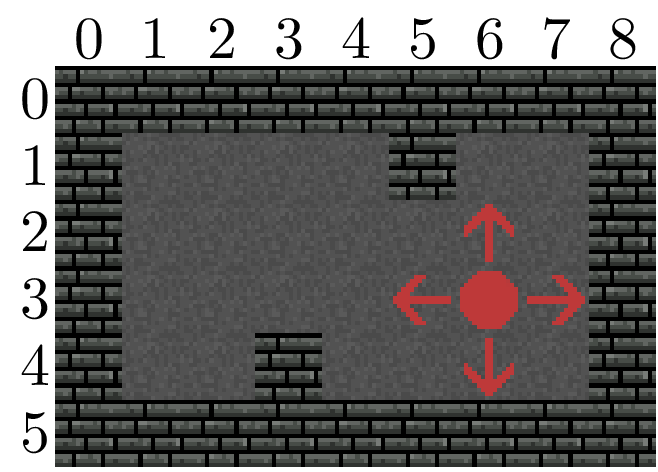
\includegraphics[width=0.9\textwidth]{rules/moves.png}};
                            \begin{scope}[x={(image.south east)}, y={(image.north west)}]
                                \draw[help lines, xstep=(1/9), ystep=(1/6)] (0,0) grid (1,1);
                                \foreach \x in {0, 1, ..., 9} { \node [anchor=north] at (\x / 10, 0) { 0.\x }; }
                                \foreach \y in {0, 1, ..., 9} { \node [anchor=east] at (0, \y / 10) { 0.\y }; }
                            \end{scope}
                        \end{tikzpicture}
                            \caption*{Déplacements autorisés}
                        \end{figure}
                    }
                    \only<3>{
                        \begin{figure}
                            \centering
                            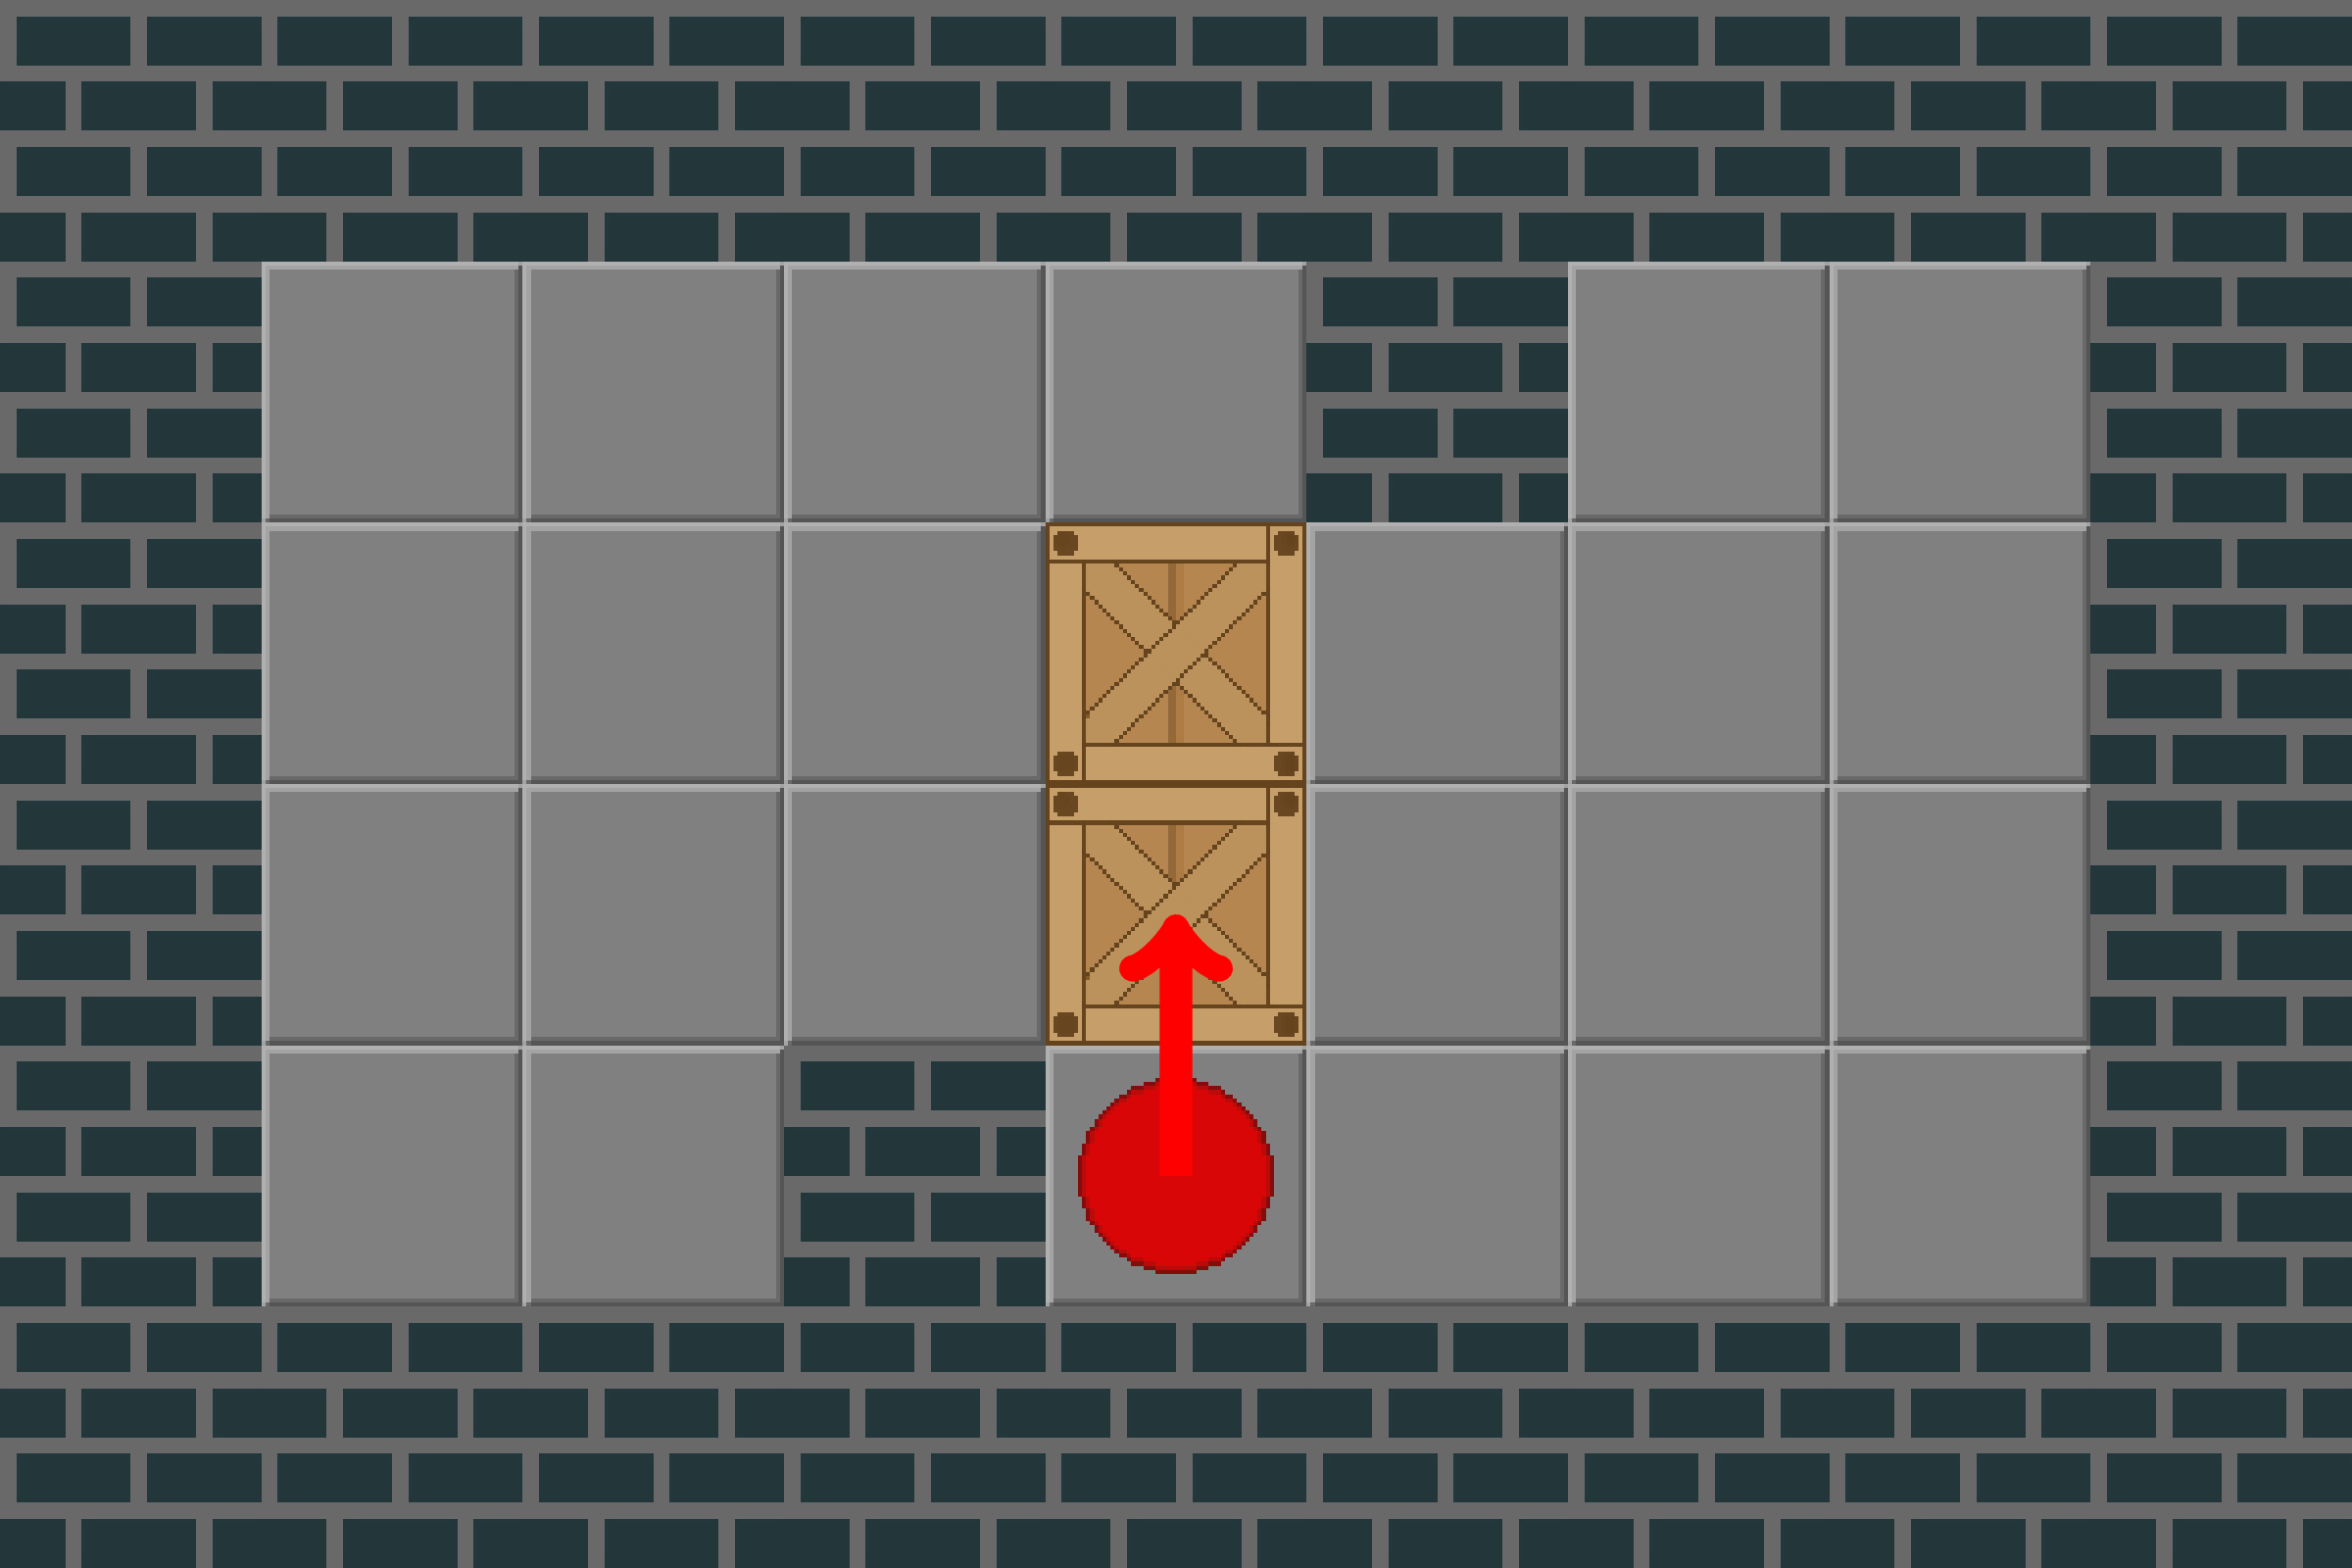
\includegraphics{rules/move_no_1.png}
                            \caption*{
\includegraphics[width=\iconwidth]{icons/no.png}}
                        \end{figure}
                    }
                \end{column}
                \begin{column}{0.5\textwidth}
                    \only<2>{
                        \begin{figure}
                            \centering
                            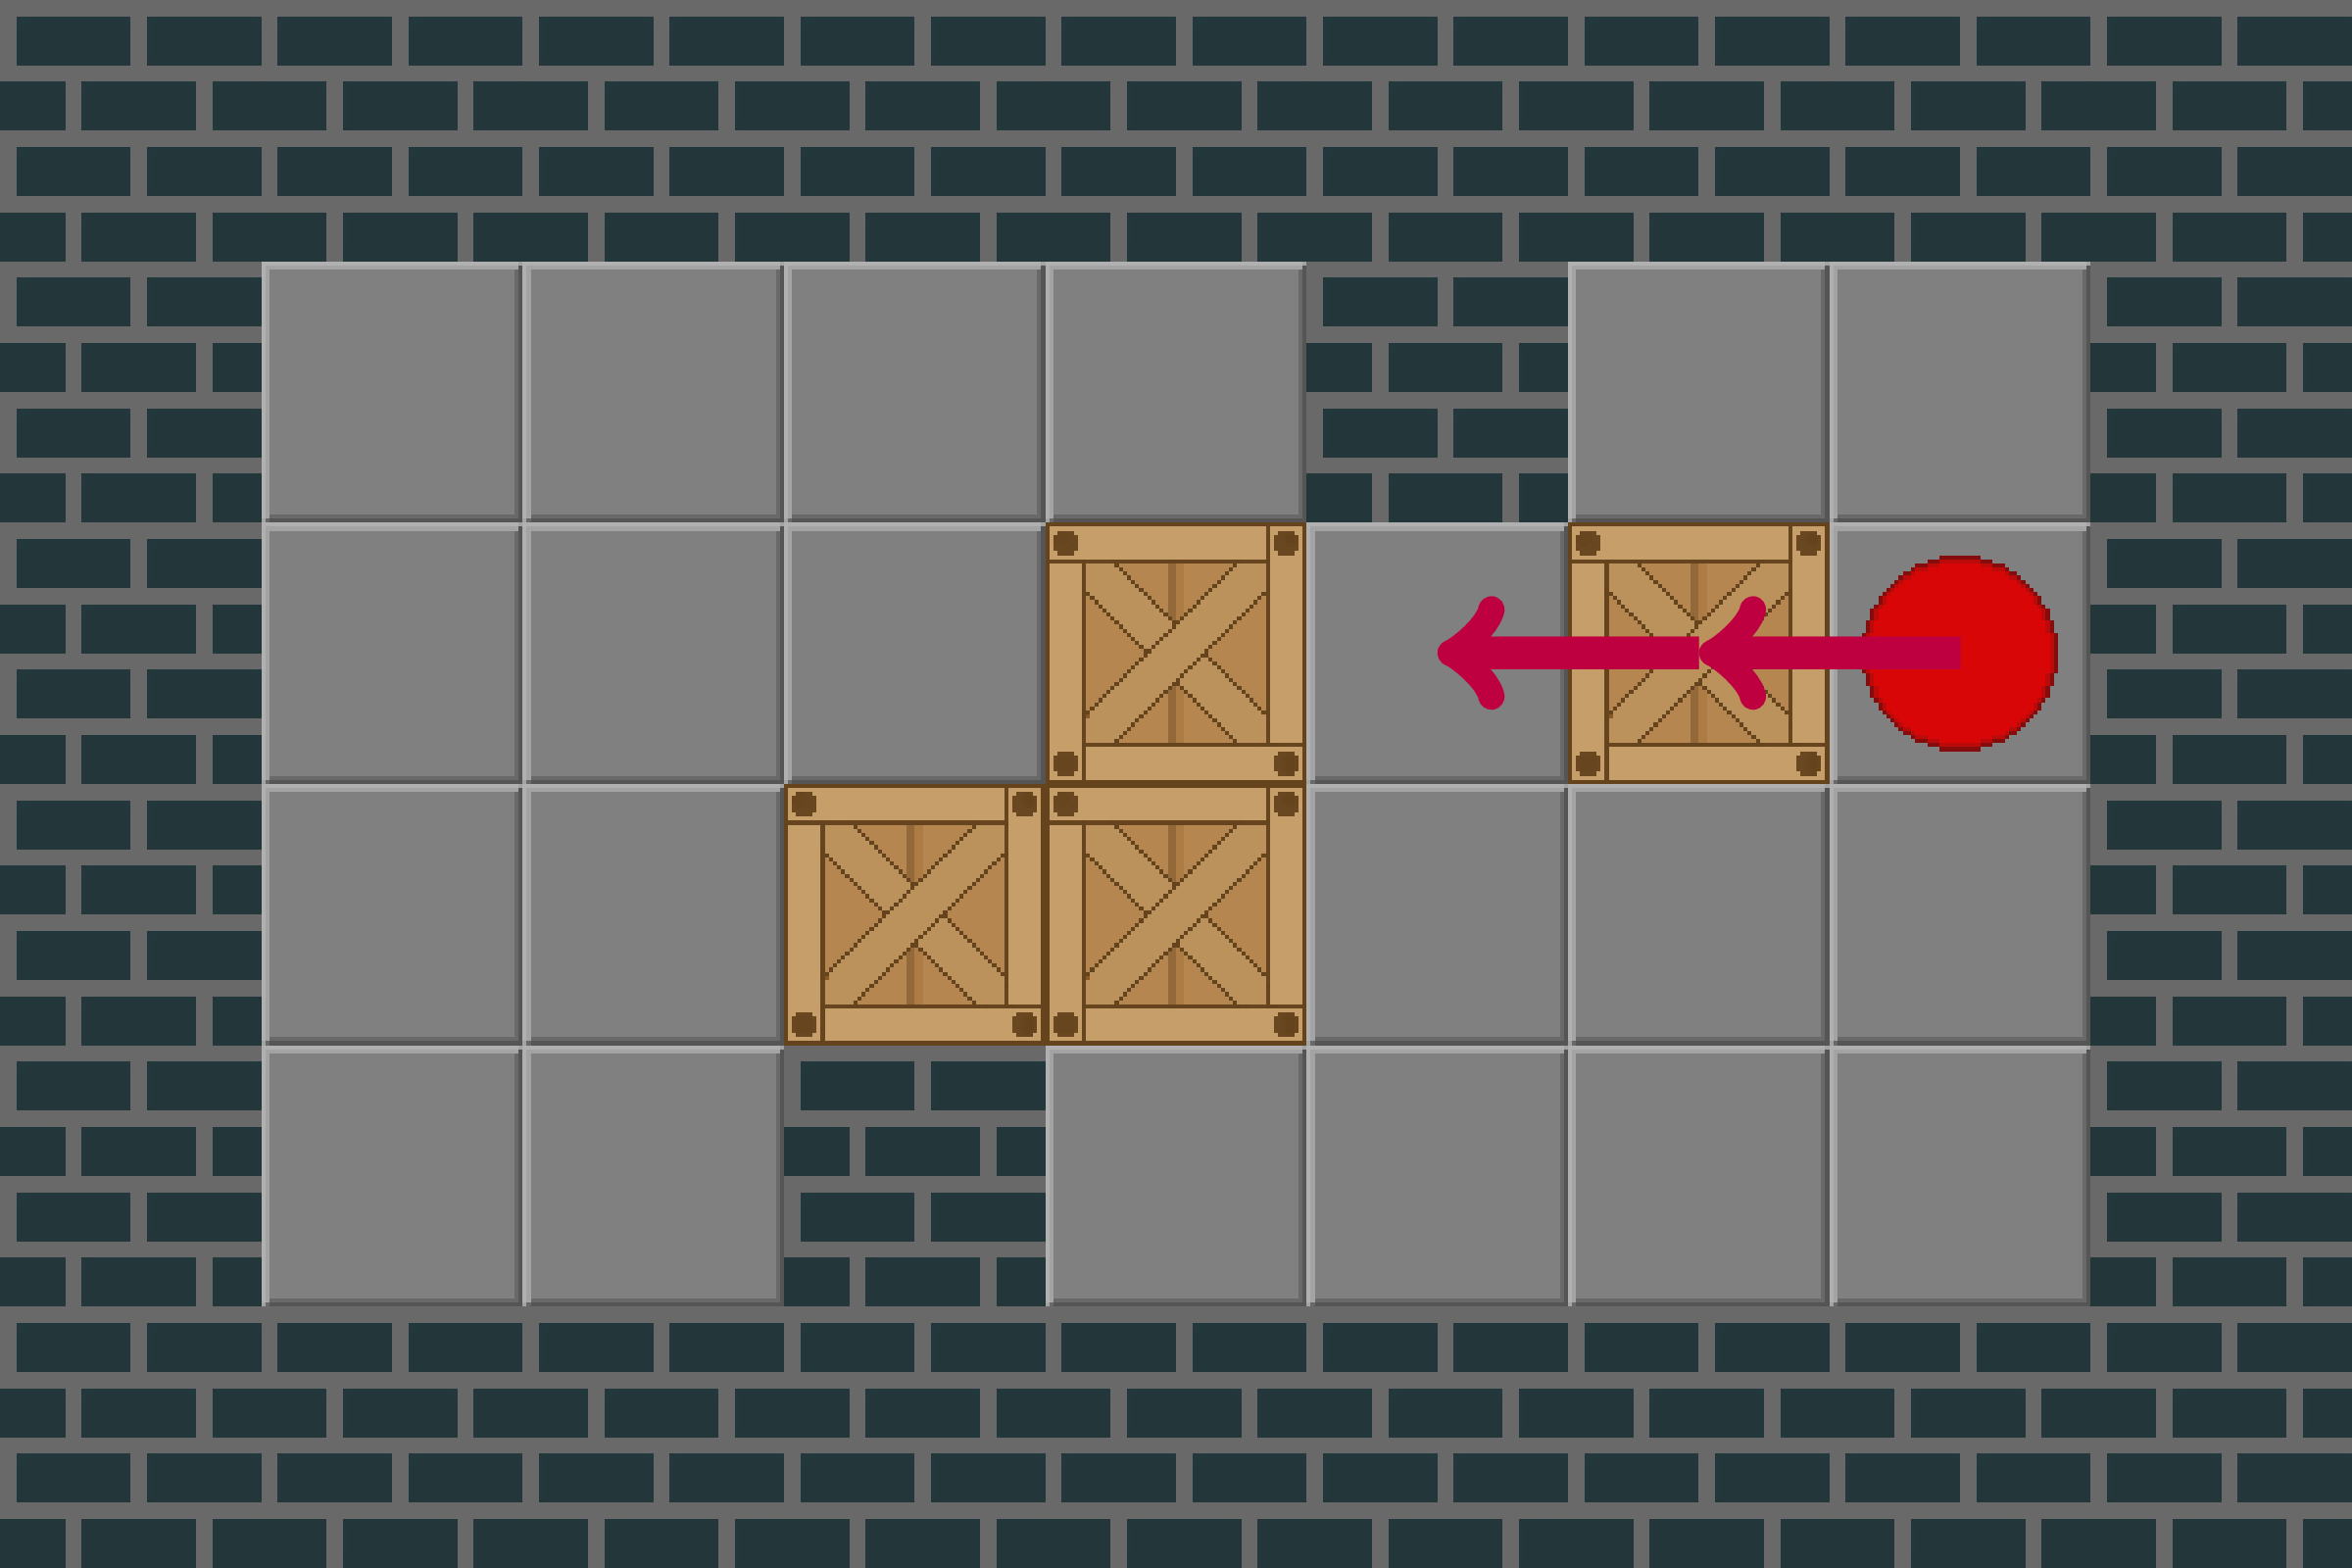
\includegraphics{rules/move_yes.png}
                            \caption*{
\includegraphics[width=\iconwidth]{icons/yes.png}}
                        \end{figure}
                    }
                    \only<3>{
                        \begin{figure}
                            \centering
                            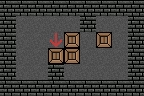
\includegraphics{rules/move_no_2.png}
                            \caption*{
\includegraphics[width=\iconwidth]{icons/no.png}}
                        \end{figure}
                    }
                \end{column}
            \end{columns}
        \end{frame}

        \begin{frame}{But du jeu}
            \centering
            \begin{columns}
                \begin{column}{0.5\textwidth}
                    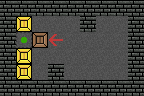
\includegraphics[width=\columnwidth]{rules/last_move.png}
                \end{column}
                \begin{column}{0.5\textwidth}
                    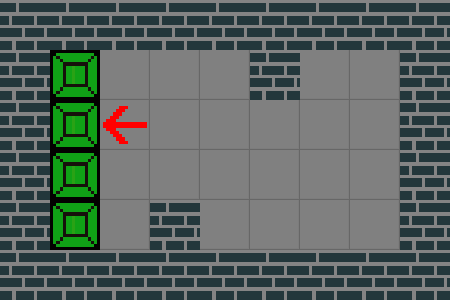
\includegraphics[width=\columnwidth]{rules/end.png}
                \end{column}
            \end{columns}
        \end{frame}

        \begin{frame}{Lien avec le thème de l'année}
            \centering
            \only<1>{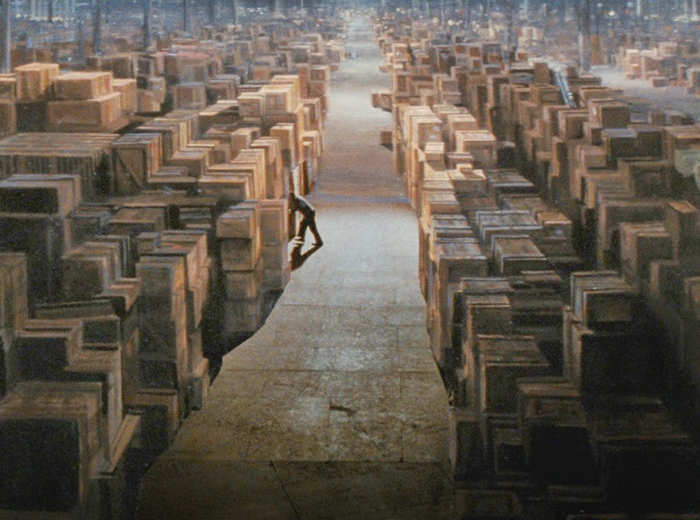
\includegraphics[width=0.9\textwidth]{warehouse.jpg}}
            \only<2>{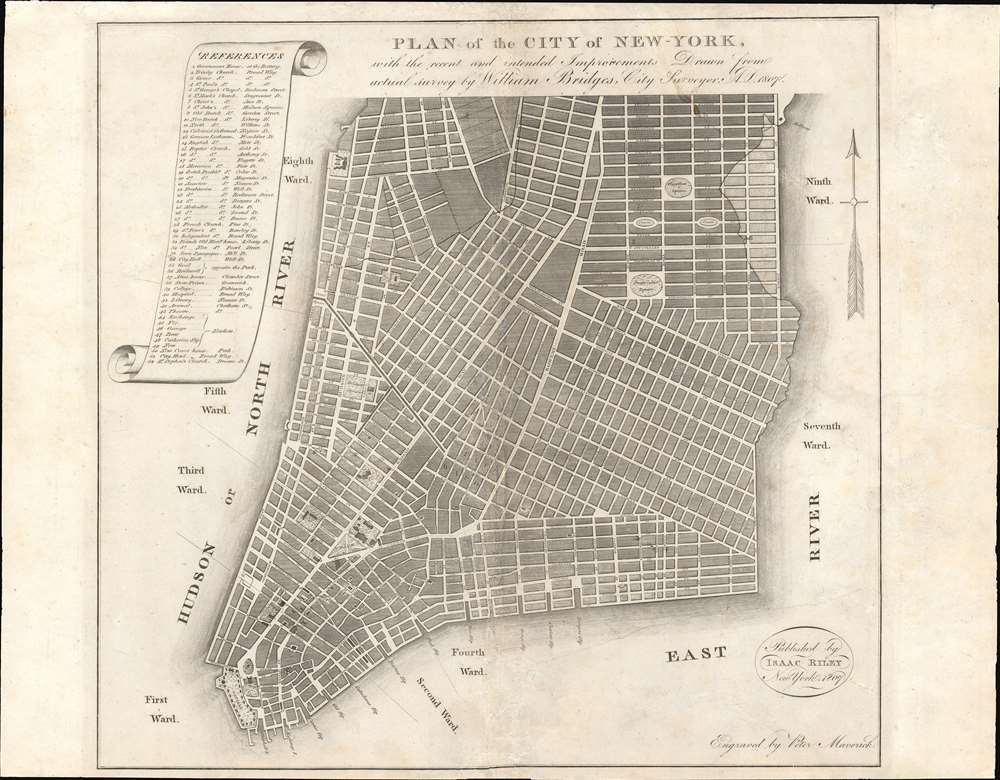
\includegraphics[width=0.9\textwidth]{city_plan.jpg}}
        \end{frame}

    \section{Principe de résolution}
            \begin{frame}{Arbre des états}
                \centering
                \begin{customtree}
                    
\node{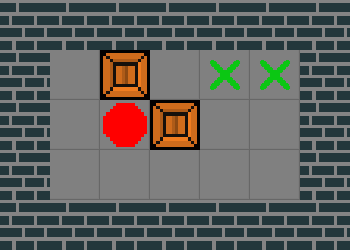
\includegraphics[width=0.3\textwidth]{exhaustive_search/1.png}}
child[visible on=<2->]{
    node{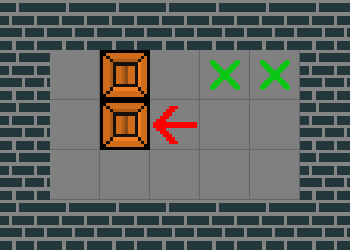
\includegraphics[width=0.3\textwidth]{exhaustive_search/1_1.png}}
    child[visible on=<4->]{
        node{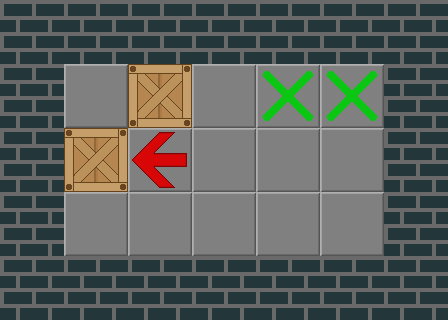
\includegraphics[width=0.3\textwidth]{exhaustive_search/1_1_1.png}}
        child[visible on=<7->]{
            node[dot]{$\dots$}
        }
    } child[visible on=<5->]{
        node{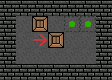
\includegraphics[width=0.3\textwidth]{exhaustive_search/1_1_2.png}}
        child[visible on=<7->]{
            node[dot]{$\dots$}
        }
    }
} child[visible on=<3->]{
    node{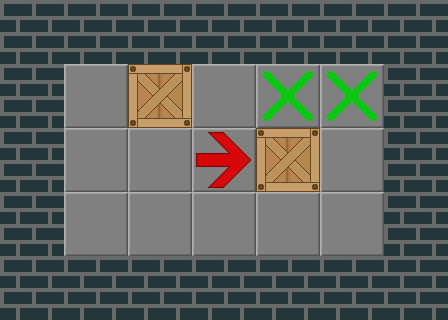
\includegraphics[width=0.3\textwidth]{exhaustive_search/1_2.png}}
    child[visible on=<6->]{
        node[dot]{$\dots$}
    }
};
                \end{customtree}
            \end{frame}

            \begin{frame}{Exemple développé}
                \begin{adjustbox}{max totalsize={\textwidth}{\textheight}, center}
                    \begin{customtree}
                        \node{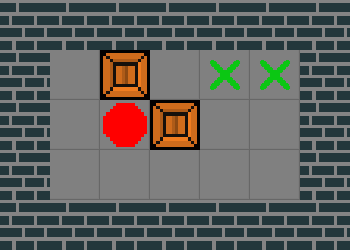
\includegraphics{exhaustive_search/1.png}}
child{
    node{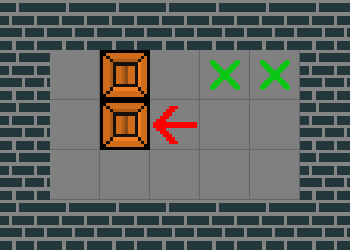
\includegraphics{exhaustive_search/1_1.png}}
    child{
        node{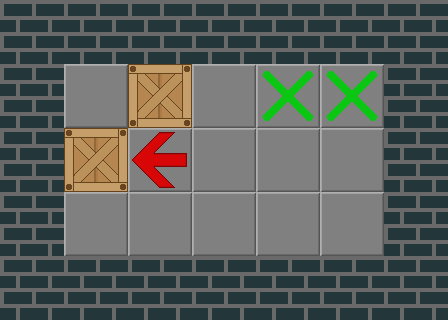
\includegraphics{exhaustive_search/1_1_1.png}}
        child{
            node[dot]{$\dots$}
        }
    } child {
        node{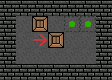
\includegraphics{exhaustive_search/1_1_2.png}}
        child{
            node(sameState1){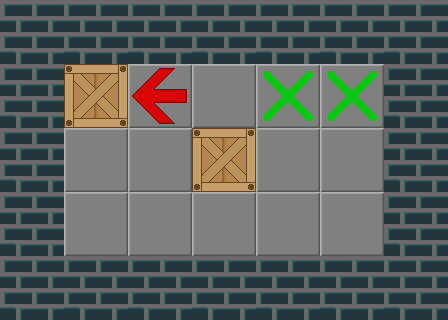
\includegraphics{exhaustive_search/1_1_2_1.png}}
            child{
                node[dot]{$\dots$}
            }
        } child{
            node(sameState2){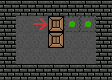
\includegraphics{exhaustive_search/1_1_2_2.png}}
            child{
                node[dot]{$\dots$}
            }
        }
    }
} child{
    node{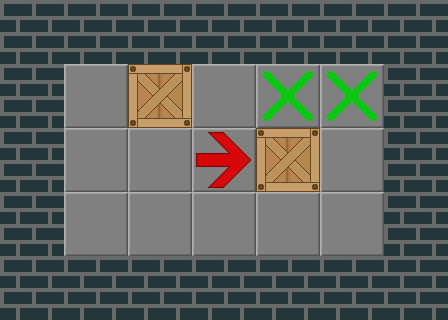
\includegraphics{exhaustive_search/1_2.png}}
    child{
        node[dot]{$\dots$}
    }
} child{
    node(sameState12){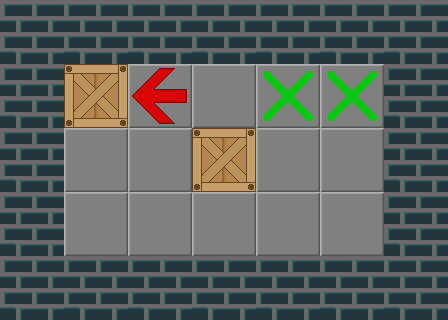
\includegraphics{exhaustive_search/1_3.png}}
    child{
        node[dot]{$\dots$}
    }
} child{
    node(sameState22){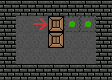
\includegraphics{exhaustive_search/1_4.png}}
    child{
        node[dot]{$\dots$}
    }
};
                    \end{customtree}
                \end{adjustbox}
            \end{frame}

            \begin{frame}{Un graphe vu comme un arbre}
                \begin{adjustbox}{max totalsize={\textwidth}{\textheight}, center}
                    \begin{customtree}
                        \node{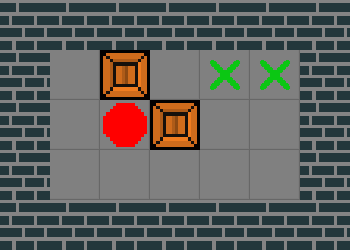
\includegraphics{exhaustive_search/1.png}}
child{
    node{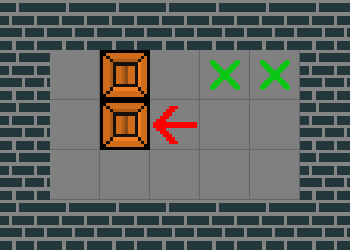
\includegraphics{exhaustive_search/1_1.png}}
    child{
        node{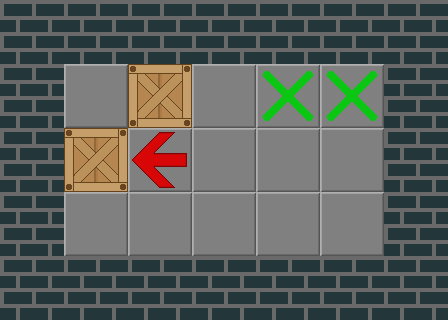
\includegraphics{exhaustive_search/1_1_1.png}}
        child{
            node[dot]{$\dots$}
        }
    } child {
        node{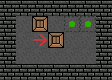
\includegraphics{exhaustive_search/1_1_2.png}}
        child{
            node(sameState1){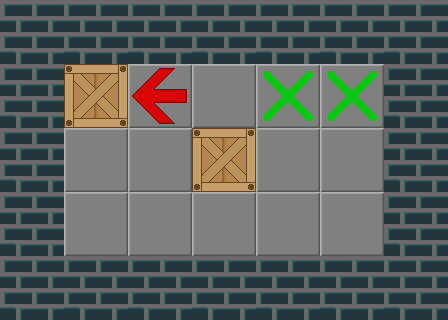
\includegraphics{exhaustive_search/1_1_2_1.png}}
            child{
                node[dot]{$\dots$}
            }
        } child{
            node(sameState2){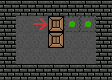
\includegraphics{exhaustive_search/1_1_2_2.png}}
            child{
                node[dot]{$\dots$}
            }
        }
    }
} child{
    node{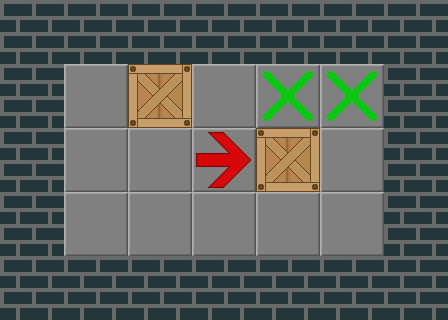
\includegraphics{exhaustive_search/1_2.png}}
    child{
        node[dot]{$\dots$}
    }
} child{
    node(sameState12){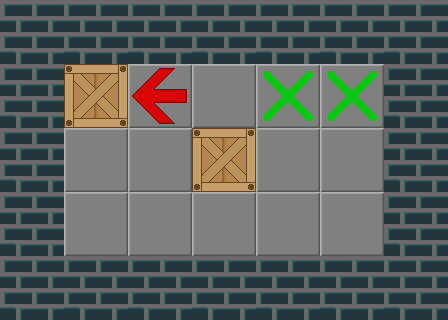
\includegraphics{exhaustive_search/1_3.png}}
    child{
        node[dot]{$\dots$}
    }
} child{
    node(sameState22){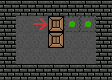
\includegraphics{exhaustive_search/1_4.png}}
    child{
        node[dot]{$\dots$}
    }
};

                        \node(c1)[draw, ellipse, minimum width=4.2cm, minimum height=3.2cm, line width=1mm, red] at (sameState1.center){};
                        \node(c2)[draw, ellipse, minimum width=4.2cm, minimum height=3.2cm, line width=1mm, red] at (sameState2.center){};
                        \node(c12)[draw, ellipse, minimum width=4.2cm, minimum height=3.2cm, line width=1mm, red] at (sameState12.center){};
                        \node(c22)[draw, ellipse, minimum width=4.2cm, minimum height=3.2cm, line width=1mm, red] at (sameState22.center){};

                        \draw[<->, draw=red, line width = 2mm] (c1.north) |- (c12.west);
                        \draw[<->, draw=red, line width = 2mm] (c2.east) -| (c22.south);
                    \end{customtree}
                \end{adjustbox}
            \end{frame}

    \section{Réduction de l'espace de recherche}

        \subsection{Analyse statique}

            \begin{frame}{Détection des positions mortes \textit{(dead positions)}}
                \centering
                \only<1>{
                    \begin{tikzpicture}
                        \node(before){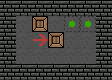
\includegraphics{dead_positions/example_before.png}};
                        \node(after)[right=of before]{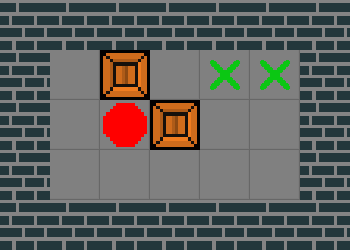
\includegraphics{dead_positions/example_after.png}};
                        \draw[->, line width=\arrowwidth] (before) -- (after);
                    \end{tikzpicture}
                }
                \only<2-> {
                    \begin{enumerate}
                        \only<2>{
                            \item
                                \begin{tikzpicture}[baseline]
                                    \node(first){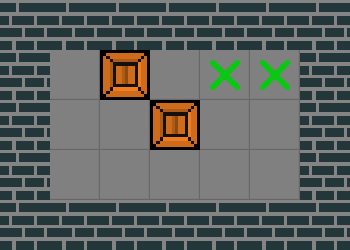
\includegraphics{dead_positions/algo_1_1.png}};
                                    \node(second)[right=of first]{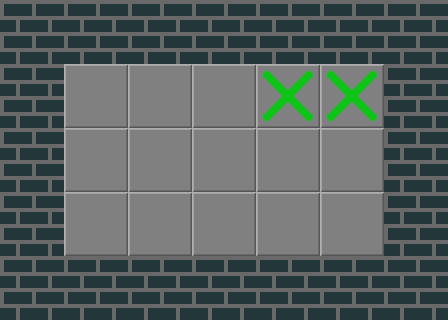
\includegraphics{dead_positions/algo_1_2.png}};
                                    \draw[->, line width=\arrowwidth] (before) -- (after);
                                \end{tikzpicture}
                        }
                        \only<3->{
                            \setcounter{enumi}{1}
                            \item
                                \begin{tikzpicture}[baseline, every node/.style={node distance=0.1cm}]
                                    \node(first){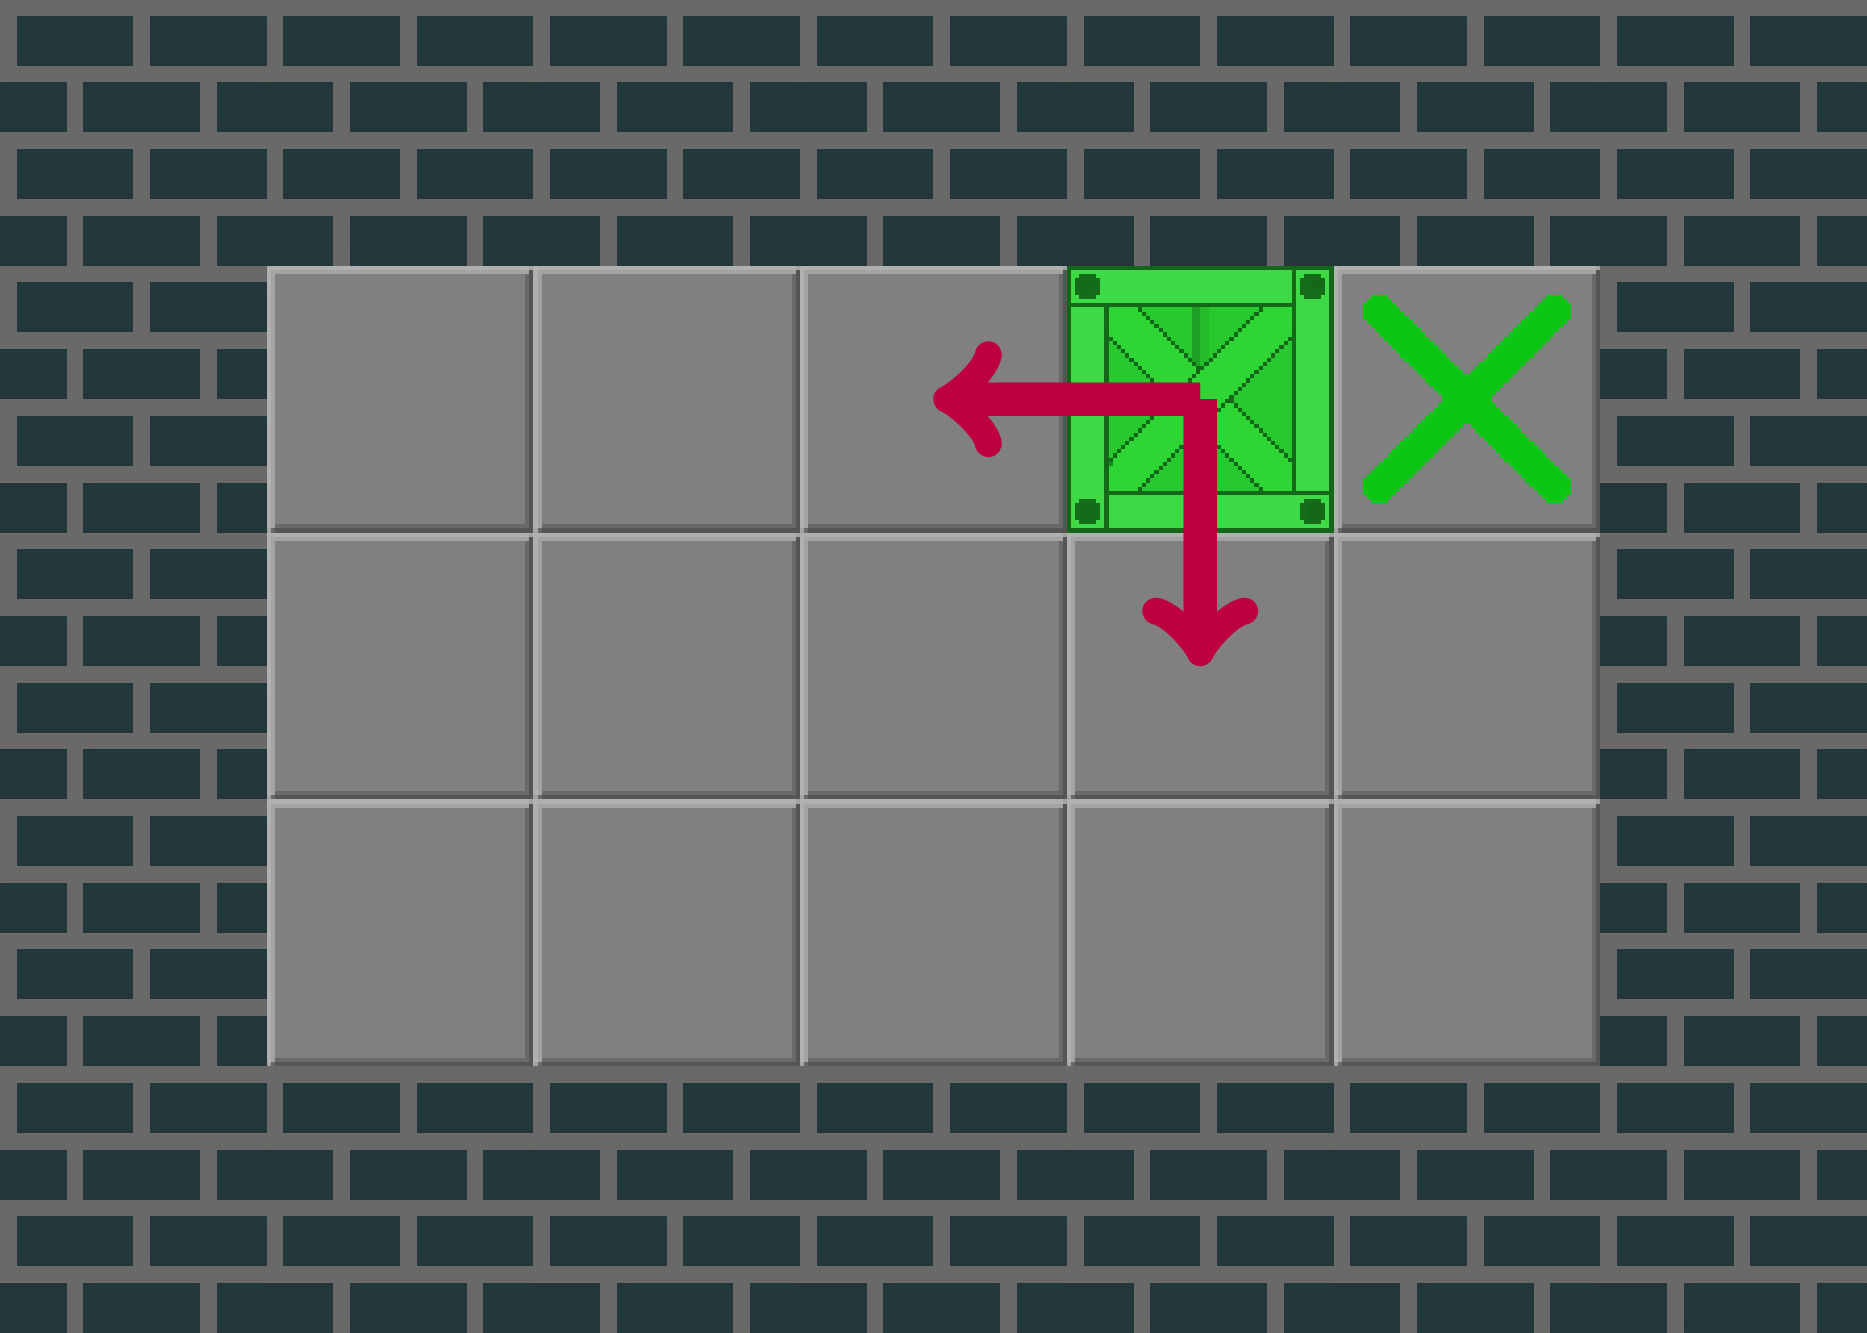
\includegraphics{dead_positions/algo_2_1.png}};
                                    \node(second)[right=of first, visible on=<4>]{$\dots$};
                                    \node[right=of second, visible on=<4>]{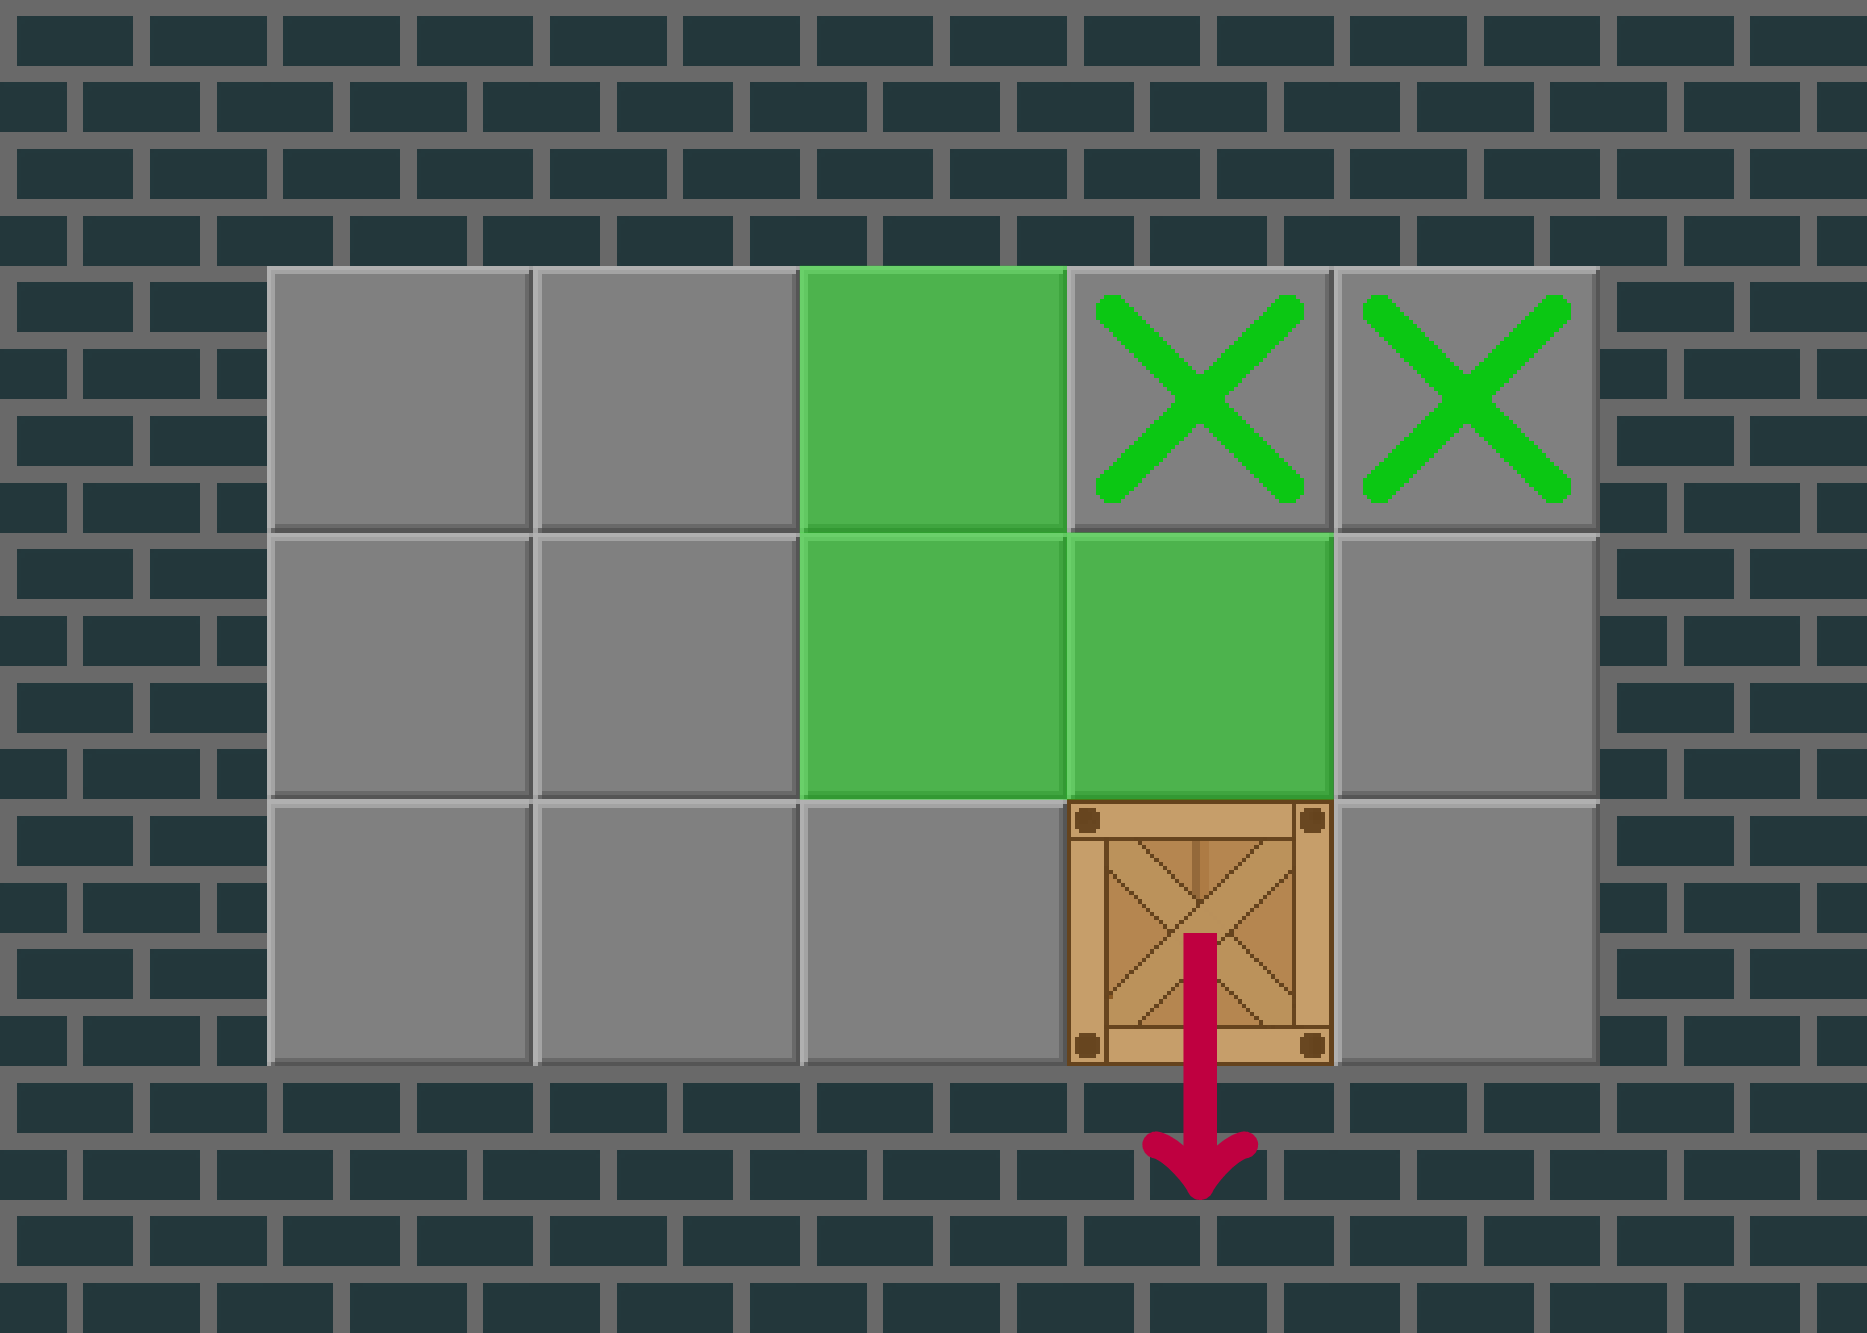
\includegraphics{dead_positions/algo_2_2.png}};
                                \end{tikzpicture}
                        }
                    \end{enumerate}
                }
            \end{frame}

            \begin{frame}{Détection de tunnels}
                \only<1>{
                    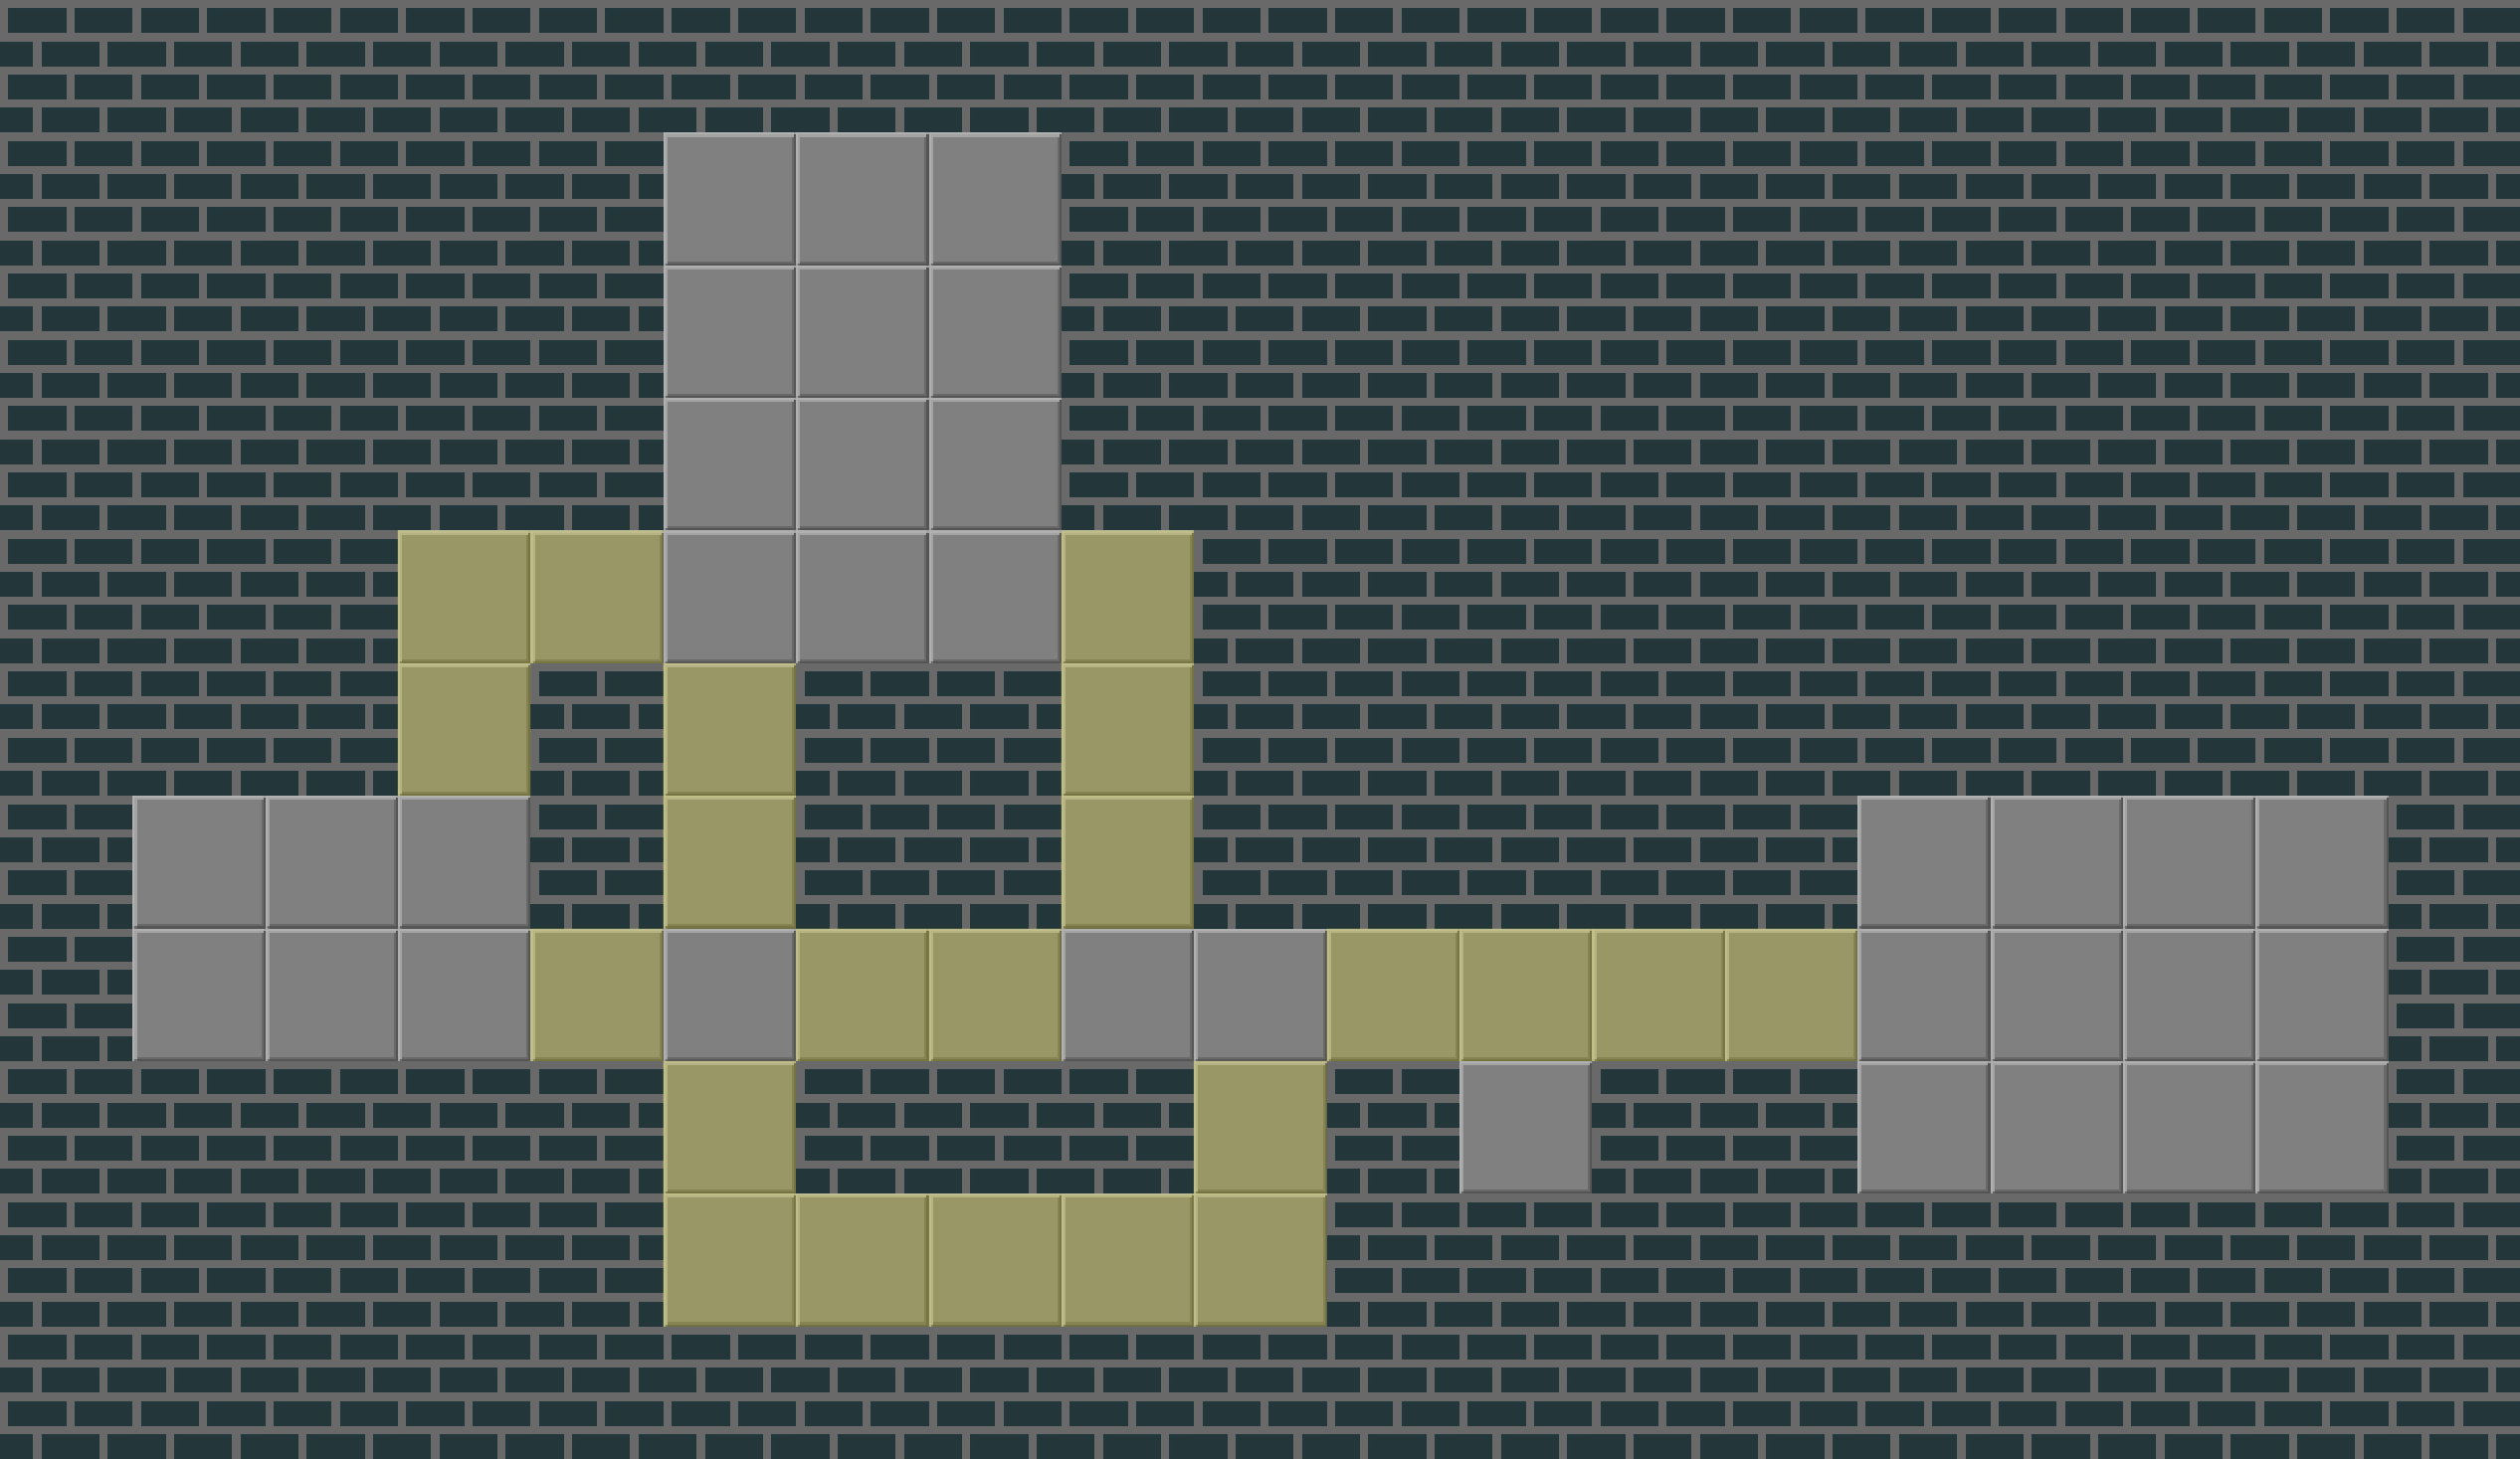
\includegraphics{tunnels/tunnels.png}
                }
                \only<2>{
                    Intérêt ? Tunnel macro !
                }
                \only<3>{
                    Parties d'un tunnel:
                    \begin{figure}
                        \centering
                        \subcaptionbox{}{
                            
\includegraphics{tunnels/straight.png}
                        }
                        \subcaptionbox{}{
                            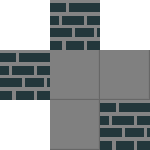
\includegraphics{tunnels/corner.png}
                        }
                    \end{figure}
                }
            \end{frame}

            \begin{frame}{Calcul d'un ordre de rangement \textit{(packing order)}}
            \end{frame}

        \subsection{Analyse dynamique}

            \begin{frame}{Détection d'impasses \textit{(deadlocks)}}
                % Ajouter un exemple simple de deaedlock ?
                \begin{figure}
                    \centering
                    \subcaptionbox{\textit{Freeze deadlock n°1}}
                        {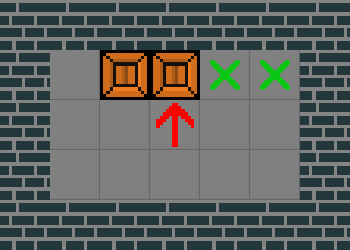
\includegraphics{freeze_deadlock/ex_1_dead.png}}
                    \subcaptionbox{\textit{Freeze deadlock n°2}}
                        {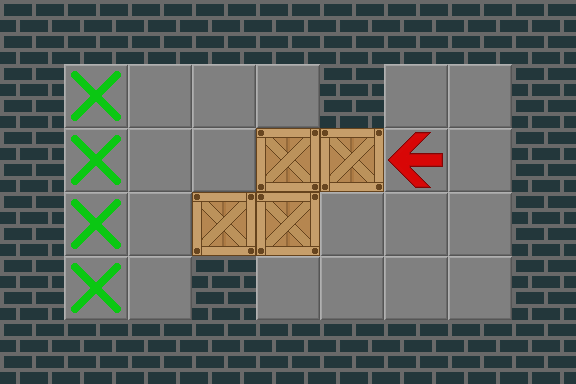
\includegraphics{freeze_deadlock/ex_2_dead.png}}
                    \subcaptionbox{\textit{PI Corral deadlock}}
                        {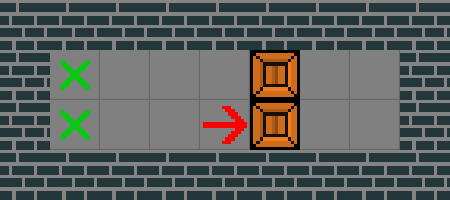
\includegraphics{pi_corral_deadlock_dead.png}}
                \end{figure}
            \end{frame}

            \begin{frame}{Détection de \textit{freeze deadlocks}}
                \begin{figure}
                    \centering
                    \subcaptionbox{Règle n°1}[.3\textwidth]
                    {
\includegraphics{freeze_deadlock/rule_1.png}}
                    \subcaptionbox{Règle n°2}[.3\textwidth]
                    {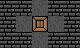
\includegraphics{freeze_deadlock/rule_2.png}}
                    \subcaptionbox{Règle n°3}[.3\textwidth] {
                        \begin{tikzpicture}
                            \node{\includegraphics{freeze_deadlock/rule_3.png}};
                            % comment mettre un point d'interrogation sur les deux caisses ajacentes à la caisse centrale?
                            % et comment centrer dans un tikzpicture?
                        \end{tikzpicture}
                    }
                \end{figure}
            \end{frame}

            \begin{frame}{Détection de \textit{freeze deadlocks}}
                \begin{center}
                    \begin{tikzpicture}
                        \node(start)                                      {\includegraphics[width=0.3\textwidth]{freeze_deadlock/ex_2_dead.png}};
                        \node(first)  [visible on=<2-4>, right=of start]  {\includegraphics[width=0.3\textwidth]{freeze_deadlock/ex_2_explanation_1.png}};
                        \node(second) [visible on=<3-4>, below=of first]  {\includegraphics[width=0.3\textwidth]{freeze_deadlock/ex_2_explanation_2.png}};
                        \node(third)  [visible on=<4-4>, left=of second]  {\includegraphics[width=0.3\textwidth]{freeze_deadlock/ex_2_explanation_3.png}}
                            child[visible on=<4-4>]{node{Gelée!}};

                        \draw[->, line width=\arrowwidth, visible on=<2-4>] (start.east)  -- (first.west);
                        \draw[->, line width=\arrowwidth, visible on=<3-4>] (first.south) -- (second.north);
                        \draw[->, line width=\arrowwidth, visible on=<4-4>] (second.west) -- (third.east);
                    \end{tikzpicture}
                \end{center}
            \end{frame}

    \section{Recherche dirigée par une heuristique}
        \begin{frame}{Heuristique simple \textit{(Simple Lower Bound)}}

            \only<1>{

            }
        \end{frame}

        \begin{frame}{Heuristique gloutonne \textit{(Greedy Lower Bound)}}
        \end{frame}

    \section{Optimisations}
        \begin{frame}{}
        \end{frame}

    \section{Résultats}
\end{document}
